\chapter{Component Selection}
This section details the process and reason for selecting each component
\section{Propulsion}

A testing rig should be designed to test the thrust of each motor-propeller assembly for two reasons:
\begin{enumerate}
	
	\item Ensures the motors are functioning
	\item Ensure the thrust from motor is within a certain tolerance
	
\end{enumerate}

An example rig can be found here, \href{https://www.banggood.com/Mayatech-MT10-10KG-Motor-Thrust-Tester-Propeller-Power-Tension-Measurement-For-RC-Model-Racing-Drone-p-1442104.html?gmcCountry=CA&currency=CAD&createTmp=1&utm_source=googleshopping&utm_medium=cpc_bgs&utm_content=yixuan&utm_campaign=ssc-ca-en-0213&gclid=CjwKCAjwmKLzBRBeEiwACCVihhjP9RAx65sLv2OFui5eUaMqfx3rBVgE6KZotZjVDXiZH75DfHi8yRoCh1EQAvD_BwE&cur_warehouse=CN}{motor testing rig}.

\subsection{Motor}
Include the desired motor specifications and possible products.
\subsection{Propeller}
There are a couple of specifications that determine the performance of the propeller. Pitch, size, the number of blades; propeller material, and propeller weight \cite{droneomega}

The pitch of a propeller is defined as the distance the propeller would move in one revolution if it were moving through a soft solid. The higher the pitch, the faster the drone will fly. This is analogous to a screw; the pitch is measured the same way. The pitch must not be too flat or too steep as this will result in no lift being generated. 

\begin{figure}[!htb]
	\graphicspath{ {Images/} }
	\centering
	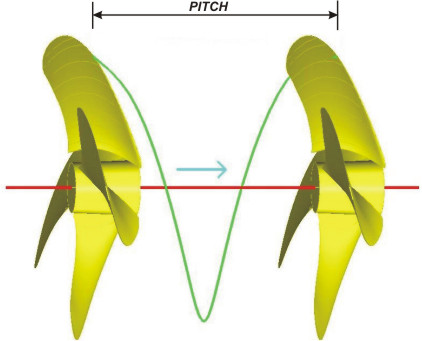
\includegraphics[width=0.6\textwidth,scale=0.8]{propeller.jpg}
	\caption{Propeller pitch }
	\label{fig:propeller}
\end{figure}

The length of the propeller from tip-to-tip is the defined as the length. Longer propellers generate more thrust for the same speed but require more torque from the motor. 

\section{Chassis}
The chassis includes the internal frame, the arms, and the landing feet. These will be made of various materials, most being 3D printed.

\hl{It might be helpful to develop a finite element model (FEM) of the top and bottom plates with the arms attached to determine optimal plate material and thickness.}

NOTE: Make a table comparing manufacturing techniques; 3D printing, injection moulding.

Look for other manufacturing techniques for landing gears and other common parts.

\subsection{Materials}
Table \ref{tab:material} shows the possible material properties which could be used for the chassis components. 

Other materials may be added and evaluated to determine if they are suitable for use in the drone. 

\begin{table*}[ht]
	\centering
	\caption[Material Properties]{\bfseries{Material properties for chassis}}
	\label{tab:material}
	\vspace{5pt}
	\begin{tabularx}{\textwidth}{Xp{2.5cm}p{2.5cm}p{2.5cm}}	
		\toprule[2pt]
		\textbf{Material} & \textbf{Density (g/cm$^3$)} & \textbf{Ultimate Strength (MPa)} & \textbf{Young’s Modulus (MPa)}\\
		\toprule[2pt]
		PA2200 Nylon – Laser Sintered & 0.93 & 48.0 & 1700 \\
		\hline
		PA1101 Nylon – Laser Sintered & 0.99 & 48.0 & 1600\\
		\hline
		PA12 Nylon – Multijet Fusion & 1.01 & 48.0 & 1800\\
		\hline
		Thermoplastic Polyurethane (TPU)$^1$ & 1.12 & 5.5 & 65 \\
		\hline
		Epoxy/Carbon Fiber Composite$^2$ & 1.4 & 878.0 & 94.6 \\
		\hline
	\end{tabularx}
\end{table*}
\noindent
$^1$This is an anisotropic material.\\
$^2$These are average values.

% need to add references

a military version could be made with a carbon fibre and kevlar blend, hardened with resin through vacuum. Propeller guards could be made the same way. 

\hl{Pros and cons of propeller guards?}

\subsection{Frame Design}
The size of the drone will depend on several factors. The size of the propellers, battery pack, and electronics. 
The frame of the drone will be constructed of 3D printed nylon parts because this allows for modularity and easy replacement of parts in the event of a failure. The type of nylon from Table \ref{tab:material} will be selected based on cost. 
The top and bottom plates will compress the arms to hold them in place,  these plates will need to be stiff? (check) and could be constructed from off the shelf carbon fiber sheets cut to the specified shape. The arms need to be held in tight between the plates, we should consider adding some vibration damping between the plates to reduce transfer to the electrical components. \hl{The manufacturer of these plates still needs to be determined.} 

Consideration should also be given to the placement of a power and reset button on the outside of the quadcopter.

\hl{List requirements for the frame design.}

\subsection{Arms}
The arms should be constructed from carbon fiber tubes. The sharp of the tubes will be selected based on the method selected to fix them to the frame, the strength of the tubes under bending, and the cost. The possible shapes are as follows:

\begin{itemize}
	\setlength{\itemsep}{0pt}%
	\setlength{\parskip}{-6pt}%
	\item Square – easier to fix to the frame and will not rotate, not as aesthetically pleasing
	\item Circular 
	\item Elliptical 
	\item Rectangular
\end{itemize}

The method for fixing the arms to the frame in order to prevent rotation is challenging. \hl{Ideas need to be generated and documented. }

\hl{List the requirements of the arms.}

\subsection{Landing Feet}
The intent in designing the landing feet is that they will be modular and can accommodate a variety of use cases. 

The feet could be placed in two different locations. Either beneath the motors at the end of the arms or near the body at the beginning of the arms. An analysis of the best location should be conducted with consideration placed on durability of body on hard landings and the landing platform.

\hl{List the different styles of feet.}

\hl{List the requirements of the feet.}

The landing feet should be 

\section{Electronics}

\subsection{Computer and Carrier Board}
The Spiri Mu uses a Nvidia TX2 for the computer and an \href{http://connecttech.com/product/asg002-elroy-carrier-for-nvidia-jetson-tx2-tx1/}{Elroy Carrier board}, which acts as a motherboard for the computer.

The reason for using this computer is it has a graphics processing unit on board so the image recognition algorithms can be run on the unit. 

ConnectTech will make the carrier board for the next generation Nvidia SOM. The new carrier board will incorporate camera input to remove the need for the camera interposers and ribbon cables. (source?)

\hl{Why was the connectech board selected?}

\subsection{Flight Controller}
The current flight controller used on the Spiri Mu is the \href{https://store.mrobotics.io/mRo-PixRacer-R14-Official-p/auav-pxrcr-r14-mr.htm}{mRo AUAV Pixracer R15}mRo AUAV Pixracer R15. The reason this was selected is …(I assume this is due to the compatibility with the GPS or vice versa)

This package contains:

\begin{itemize}
	\setlength{\itemsep}{0pt}%
	\setlength{\parskip}{-6pt}%
	\item Invensense ICM-20608-G 3-axis accelerometer/gyroscope
	\item Invensense MPU-9250 3-axis accelerometer/gyroscope/magnetometer 
	\item MEAS MS5611 barometer
	\item Honeywell HMC5983 magnetometer temperature compensated
\end{itemize}

\subsection{Electronic Speed Controller}
For small drones,  4-in-1 ESC's are appropriate. For larger drones \hl{(what does larger mean in this case?)}, one ESC per motor would be required \hl{(why? I assume more power output)} 

Large drones (in our case) may have 8 motors, one up and one down on each of four arms.

\subsection{GNSS/Compass}
The GPS and compass used on the Spiri Mu is the \href{https://store.mrobotics.io/mRo-GPS-u-Blox-Neo-M8N-Dual-Compass-LIS3MDL-IST831-p/mro-gps003-mr.htm}{mRo GPS u-Blox Neo-M8N}. 

For the next generation, the RTK GPS available from MRo, which greatly improves position accuracy. \hl{What are the differences from the current one? How much more accurate is it?}

\subsection{Optical Components}
The optical components are the cameras and the range finder.

The camera units currently used on the Spiri Mu is two \href{https://leopardimaging.com/product/cmos-sensor-modules/mipi-camera-modules/li-m021c-mipi/}{LI-M021C-MIPI} . Another camera unit is being considered which is the the AR0144 \hl{provide link}

An IR sensor could also be added to the array. \hl{what benefit does this provide}

The reason for this is that we want direct CSI input for the built in cameras, not a USB interface. \hl{what are the benefits to using CSI over USB?}

\subsection{Power}
The battery pack should incorporate a step-down converter and 5 cells. \hl{why 5 cells? why not 6 cells?}
\noindent
The battery pack should have the following characteristics:
\begin{itemize}
	\setlength{\itemsep}{0pt}%
	\setlength{\parskip}{-6pt}%
	\item Easily changed with a clip mechanism
	\item Connected to the drone using blade type connectors
	\item Fixed 15.5V
	\item Ability to supply 40A
	\item Spot welded connections between cells
	\item Balance charging
\end{itemize}

Hot-swapping batteries and moving batteries from one drone to the other should be possible.

\subsection{Power Management}
The power management system consists of the power distribution board.

\subsection{Modular Payloads}
\noindent
The drone will be designed to carry a variety of different payload masses. These could include:
\begin{itemize}
	\setlength{\itemsep}{0pt}%
	\setlength{\parskip}{-6pt}%
	\item FLIR Camera + gimbal
	\item Water testing equipment
	\item Normal camera + gimbal
	\item Agricultural multi-spectral sensor
	\item LIDAR
\end{itemize}
\hl{Need to know whether each needs a custom bottom shell}

\section{Overall Construction}
Overview of properties for the entire drone. \\

\hl{Would be a good idea to make requirements for each subsection then requirements for the overall drone.}\\

\hl{This section will include a wiring diagram to be added later.}\\